%
% File acl2020.tex
%
%% Based on the style files for ACL 2020, which were
%% Based on the style files for ACL 2018, NAACL 2018/19, which were
%% Based on the style files for ACL-2015, with some improvements
%%  taken from the NAACL-2016 style
%% Based on the style files for ACL-2014, which were, in turn,
%% based on ACL-2013, ACL-2012, ACL-2011, ACL-2010, ACL-IJCNLP-2009,
%% EACL-2009, IJCNLP-2008...
%% Based on the style files for EACL 2006 by 
%%e.agirre@ehu.es or Sergi.Balari@uab.es
%% and that of ACL 08 by Joakim Nivre and Noah Smith

\documentclass[11pt,a4paper]{article}
\usepackage[hyperref]{acl2020}
\usepackage{times}
\usepackage{latexsym}
\renewcommand{\UrlFont}{\ttfamily\small}
\usepackage{graphicx}
\graphicspath{ {./figures/} }

% This is not strictly necessary, and may be commented out,
% but it will improve the layout of the manuscript,
% and will typically save some space.
\usepackage{microtype}

%\aclfinalcopy % Uncomment this line for the final submission
%\def\aclpaperid{***} %  Enter the acl Paper ID here

%\setlength\titlebox{5cm}
% You can expand the titlebox if you need extra space
% to show all the authors. Please do not make the titlebox
% smaller than 5cm (the original size); we will check this
% in the camera-ready version and ask you to change it back.

\newcommand\BibTeX{B\textsc{ib}\TeX}

\title{Son Pham at SemEval-2022 Task 4: Predicting Patronizing and Condescending Language}

\author{First Author \\
  Affiliation / Address line 1 \\
  Affiliation / Address line 2 \\
  Affiliation / Address line 3 \\
  \texttt{email@domain} \\\And
  Second Author \\
  Affiliation / Address line 1 \\
  Affiliation / Address line 2 \\
  Affiliation / Address line 3 \\
  \texttt{email@domain} \\}

\date{}

\begin{document}
\maketitle
\begin{abstract}
This document outlines the work done for the SemEval-2022 16th International Workhsop on Semantic Evaluation task 4: Patronizing and Condescending Language Detection. A set of pre-labeled patronizing and condescending language (PCL) data from the Don't Patronize Me! dataset was used to build a neural network model that can predict when a given sentence or paragraph contains patronizing and/or condescending language. Using a pre-trained text embedding model, the author performed transfer learning to fine-tune a new model for application towards the PCL context. Ultimately, the model resulted in a best validation precision score of 0.4190, validation recall score of 0.4422, and a F1 score of 0.430.

\end{abstract}

\section{Credits}

The dataset Don't Patronize Me! is credited to Carla Perez Almendros from Cardiff University. The pretrained text embedding model is made avaiable by Google and the Tensorflow 2 Hub.

\section{Introduction}

This task is aimed at building a model that can predict patronizing and/or condescending languages written in news articles or other written sources. People all tend to speak in patronizing and condescending languages, especially when speaking about particular groups such as minorities, the homeless, and the vulnerable communities. Although this type of language is common in written text, especially news articles about such "vulnerable" groups, often people do not realize that they are doing so. This task was developed to bring to light these involuntary and unconsciously spoken and/or written PCL and how one can detect when such language occurs. \cite{perez-almendros-etal-2020-dont}

% What is the main strategy your system uses? ~1 paragraph
The main strategy of this system utilizes a neural network with a series of fully connected layers built upon a pre-trained text embedding model developed by Tensorflow 2. The Pre-trained model is a token based text embedding trained on the English Google News 7B corpus (https://tfhub.dev/google/nnlm-en-dim50-with-normalization/2), which is based on a feed-forward neural netowrk language model with pre-built OOV. The model allows a mapping from text to 50-dimensional embedding vectors. With trainable settings active, the embedding layer is fed into a sequential model, which is then followed by a series of dropouts and dense layers. The final output layer consists of a sigmoid activation function to determine whether the sentence or paragraph contains any PCL (positive) or not (negative). 

% What did you discover by participating in this task? Key quantitative and qualitative results, such as how you ranked relative to other teams and what your system struggles with. ~1 paragraph
One problem that was uncovered while working on this task was the difficulty of training the model based on the given dataset. Although the labels were categorized from 0 to 4, which were then binned into either non-PCL (0-1) and PCL (2-4), there were still a significantly larger set of non-PCL samples, which proved to be difficult to train with. Quantitatively, the author's different models were returning F1 scores from about 0.2 to 0.4, and by modifying various hyperparameters, there was a bouncing back and fourth between gaining and losing from validation precision and from validation recall. Qualitatively, the author was able to correctly label over a third of the samples correctly and consistently.

\section{Background}
% In your own words, summarize important details about the task setup: kind of input and output (give an example if possible); what datasets were used, including language, genre, and size. If there were multiple tracks, say which you participated in.
As discussed above, the dataset used developed by Carla Perez Almendros et. al. named the Don't Patronize Me! dataset. The dataset is in English, 3MB in size, and contained paragraphs with annotated labels from 0 (not containing PCL) to 4 (containing highly patronizing and condescending languages). In the dataset, there are 10469 samples total, with 9620 samples non-PCL and 849 containing PCL (after binary binning). The features include a unique id for each paragraph in the corpus, a document id referencing the original News on Web corpus outlined in the README, a keyword search term that was used to retrieve texts about a target community, a country code referencing the country code of the source media outlet, the text paragraph for analysis, and the classified labels for each sample. 

% Here or in other sections, cite related work that will help the reader to understand your contribution and what aspects of it are novel.




\section{System Overview}
% Key algorithms and modeling decisions in your system; resources used beyond the provided training data; challenging aspects of the task and how your system addresses them. This may require multiple pages and several subsections, and should allow the reader to mostly reimplement your system’s algorithms.

As mentioned above, this system uses a pre-trained model as the initial layer for training. Several different pre-trained models were used during the training process, but the author ultimately used the Tensorflow 2 text embedding. This allowed the author to build upon what has been developed by Google based on the English Google News of 7 billion words corpus. The selected pre-trained model has an output shape of 50-dimensions, and was set as trainable at initialization. The pre-trained model was set up as a KerasLayer model, which wraps the SavedModel object into a Keras layer to be used subsequently. 

During the training process, a callback is set to monitor validation recall, and saving the best model that provided the highest value. The author chose recall instead of precision because it seems that when precision is high, recall gravitates significantly lower, but if recall is high, precision can be more easily tuned to get better results. 

Figure \ref{fig:model_graph} shows a graph of the neural network layers used. The model is initialized with a sequential layer. This allows building a model by sequential linear stack of layers built on top of one another. The previously mentioned pre-trained model is added to the model as the first layer, which contains 48,190,600 parameters with an output shape of 50 units. Afterwards, a dropout layer is added containing the same output shape. This layer, used to prevent overfitting, randomly changes input values to zero with a frequency of rate given as a hyperparameter. In this case, a rate of 0.4 was used. Since this changes the total sum of all inputs, all other inputs not set to zero will be increased by 1 / (1-rate). 

\begin{figure}[t]
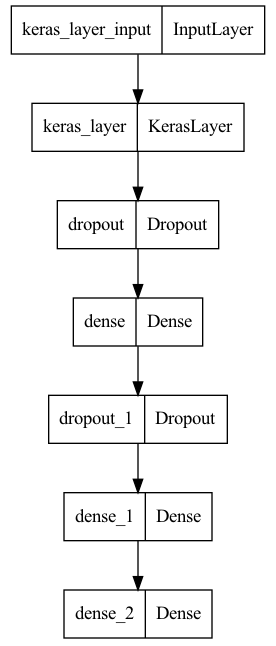
\includegraphics[scale=0.35]{model_graph.png}
\centering
\caption{Model Graph}
\label{fig:model_graph}
\end{figure}

The next layer consists of a fully connected dense layer with 50 times 20 units, resulting in 51,000 parameters with an output shape of 1000 units. This layer has a "ReLU" activation function, setting the node value to zero of the output is less than zero, or itself if equal to zero or larger. Since the network needs some pre-defined weights to start the training,for this layer, the kernel initializer was set to "HeNormal". This initializes the kernel by drawing samples from a truncated normal distribution centered on zero, with the standard deviation being std = sqrt(2/inputshape), where inputshape is the weight tensor length. 

A second dropout layer is added subsequently in order to further decrease overfitting. The same dropout frequency rate of 0.4 was used. The next layer is an additional fully connected dense layer using the same set of hyperparameters as the first dense layer. Finally, the last layer is the output layer, which takes in the previous dense layer and outputs a single value based on the sigmoid function. The number of parameters for the final layer is 1001 with an output shape of 1. The total number of parameters is 49,243,601.

Besides the pre-trained model from Google, the author relied solely on the Don't Patronize Me! dataset without any data augmentation from external sources. The most challenging aspect of this task is the unbalanced samples for PCL and non-PCL. This made it difficult for the author to find fine-tuning hyperparameter settings that allowed for both high recall and precision. One solution that helped mitigate this issue was by binning the different unique categories from the class (0-4), which was done by the SemEval team. Another technique used was to decrease the batch size for each epoch run. This allowed for increased generalization when training, which may prevent overfitting and may lead to higher accuracy. A third solution to solve the overfitting problem is to add dropout layers with relatively high dropout rates, which forces the model to not be dependent entirely on a layers output nodes and must learn with a percentage of them missing.

% Use equations and pseudocode if they help convey your original design decisions, as well as explaining them in English. If you are using a widely popular model/algorithm like logistic regression, an LSTM, or stochastic gradient descent, a citation will suffice—you do not need to spell out all the mathematical details.

% Give an example if possible to describe concretely the stages of your algorithm.

% If you have multiple systems/configurations, delineate them clearly.

% This is likely to be the longest section of your paper.


\section{Experimental Setup}
% How data splits (train/dev/test) are used.

% Key details about preprocessing, hyperparameter tuning, etc. that a reader would need to know to replicate your experiments. If space is limited, some of the details can go in an Appendix.

% External tools/libraries used, preferably with version number and URL in a footnote.

% Summarize the evaluation measures used in the task.

% You do not need to devote much—if any—space to discussing the organization of your code or file formats.

For this task, the SemEval team provided the author with the data parsing and loading functionalities, which were used through the preprocessing and evaluation sessions. Initally, the dataset was loaded manually and split into a test and training set. The author created a random train and test set splitting function based on a random indices generator that was used initially. For the remaining training sessions, the author used the selected training and development sets already segmented and parsed the indices from those to generate the model's training and testing set. After splitting, the test set was set aside for validation and evaluation. Two lists of saved indices, one for training and one for the testing sets, and used those to split the training data loaded by the SemEval script. Throughout the model training, the dev set was used as the validation set, and subsequently used as the evaluation set where results were then recorded and submitted for the practice round. 

Since the SemEval performed much of the pre-processing, the author did not need to perform any additional preprocessing. For hyperparameterization, the main tuning parameters consists of the shape of the pre-trained token embedding model, the dropout frequency rates, and the shape of the dense layers. During the fitting of the model, one can also vary the number of epochs ran and the batch size for each run. 

For this training model, the following toolsets were used: Numpy and Pandas were used for data parsing, manipulating, and for storing data as arrays and DataFrames. Tensorflow 2.7.0 and Keras were used as the main modeling engine, with the Tensorflow hub, version 0.12.0, providing the pre-trained model discussed above. Within Tensorflow, the Sequential, Dense, Dropout, and KerasLayer were used. Various visualization tools were used, particularly tensorflow's plotmodel function to generate the model graph.

To evaluate the model, the accuracy, precision, and recall were stored when compiling the combined model. Accuracy provided the author with the percentage of samples that were correctly labeled overall. Precision provided the author with the model's ability to identify relevant (true positive) data points versus the number of both true positives and false positives. The recall provided the author with the number of true positives versus the number of true positives plus the number of false negatives. After training, the model then predicts the testing dataset, which were ultimately used for scoring and submission. The main metrics are precision, recall, and F1 scores.


\section{Results}
% Main quantitative findings: How well did your system perform at the task according to official metrics? How does it rank in the competition?

% Quantitative analysis: Ablations or other comparisons of different design decisions to better understand what works best. Indicate which data split is used for the analyses (e.g. in table captions). If you modify your system subsequent to the official submission, clearly indicate which results are from the modified system.

% Error analysis: Look at some of your system predictions to get a feel for the kinds of mistakes it makes. If appropriate to the task, consider including a confusion matrix or other analysis of error subtypes—you may need to manually tag a small sample for this.

During the practice phase of the competition as of December 13, 2021, the author is currently ranked 7th based on precision (0.4190), 14th based on recall (0.4422), and 12th based on F1 score (0.430). Several different pre-trained models were used with varying fine-tuned parameters during the study. Table \ref{models_list} lists a few of the models used (based on the fine-tuning from the submitted model) and their results. Note that the trained model with the best validation recall score were used, which may or may not be the best overall for that particular run. Although Model 5 had a higher F1 score, the author was not sure if SemEval is more interested in the precision of the model versus the recall, so Model 1 was selected.

Looking at the table, one can see that the different pre-trained models provided relatively consistent results, with the 20-dimensional models having a slighly lower score due to the lowness of the available features. This causes an issue for paragraphs that contains more than 20 words, since any words greater than 20 are discarded when being input into the model. It was better to have a higher dimension and pad the empty trailing text than discarding them. The table shows that 50-dimensions are adequate for receiving good results and are not too far from 128-dimensional results. This allow for better training performance while maintaining consistent evaluation metrics values. 

\begin{table*}
\centering
\begin{tabular}{lllll}
\hline
\textbf{Model No.} & \textbf{Pre-trained Model} & \textbf{(Precision)} & \textbf{(Recall)} & \textbf{(F1)} \\
\hline
Model 1 (submitted) & nnlm-en-dim50-with-normalization & 0.419 & 0.442 & 0.430 \\
Model 2 & gnews-swivel-20dim & 0.504 & 0.286 & 0.365 \\
Model 3 & gnews-swivel-20dim-with-oov & 0.554 & 0.281 & 0.373 \\
Model 4 & nnlm-en-dim128 (google) & 0.383 & 0.477 & 0.425 \\
Model 5 & nnlm-en-dim128 (tf2-preview) & 0.358 & 0.568 & 0.439 \\
Model 6 & nnlm-en-dim128-with-normalization & 0.409 & 0.427 & 0.418 \\
\hline
\end{tabular}
\caption{\label{models_list}
List of Models Tested (with Model 1 as Baseline)
}
\end{table*}

The data split used for the training and development set was based on the functions provided by the SemEval team. The sample indices for the training and testing sets were predefined and given in a text file. Once the actual testing dataset has arrived, the prediction will be performed and results computed. Figure \ref{fig:conf_mat} shows the confusion matrix of Model 1. Here the viewer can see accuracy was high, but since there were so few samples that did contain PCL, precision and recall has more weight in the overall evaluation.

\begin{figure}[t]
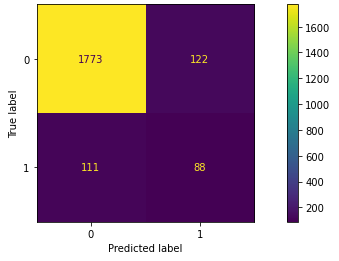
\includegraphics[scale=0.5]{conf_mat.png}
\centering
\caption{Confusion Matrix for Model 1}
\label{fig:conf_mat}
\end{figure}

Figure \ref{fig:plot_accuracy} shows the model's accuracy versus the epochs for both the training and validation sets. Figure \ref{fig:plot_loss} shows the model's loss versus the epochs. These two figures show that overfitting is a big issue in training. as the training accuracy increases, the validation accuracy decreases at first and remains constant as the epochs increase. Looking at the loss figure, one can see the validation loss continuously increase as epochs increase. As previously mentioned, methods to decrease overfitting was implemented as best as possible, but the overfit still remain relatively high. 

\begin{figure}[t]
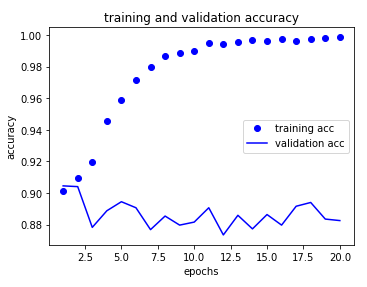
\includegraphics[scale=0.5]{plot_accuracy.png}
\centering
\caption{Accuracy for Training and Validation Set (Model 1)}
\label{fig:plot_accuracy}
\end{figure}

\begin{figure}[t]
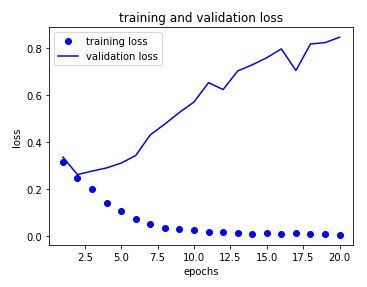
\includegraphics[scale=0.5]{plot_loss.png}
\centering
\caption{Loss for Training and Validation Set (Model 1)}
\label{fig:plot_loss}
\end{figure}

Figure \ref{fig:plot_prec} shows the model's precision score for the training and validation sets. Figure \ref{fig:plot_rec} shows the model's recall score for the sets. Here, one can see the training precision and recall increases at first, but then levels out near epoch 7, while the precision and recall for the validation set remains relatively constant. Both hovers near the 0.4 mark.

\begin{figure}[t]
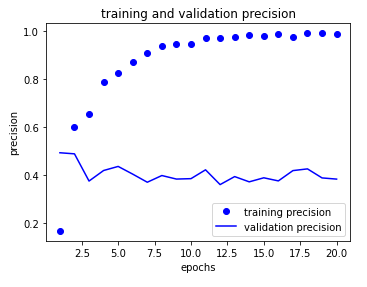
\includegraphics[scale=0.5]{plot_prec.png}
\centering
\caption{Precision for Training and Validation Set (Model 1)}
\label{fig:plot_prec}
\end{figure}

\begin{figure}[t]
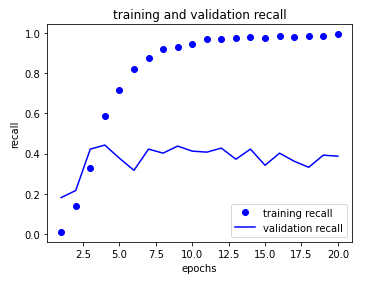
\includegraphics[scale=0.5]{plot_rec.png}
\centering
\caption{Recall for Training and Validation Set (Model 1)}
\label{fig:plot_rec}
\end{figure}


\section{Conclusion}
% A few summary sentences about your system, results, and ideas for future work.
The results presented show that with a baseline neural network using a pre-trained model, it was possible to get an F1 score of 0.4. Several different pre-trained models were used in the study to determine the variance of scores based on the text embeddings used, which showed that they remain relatively similar and the only major effect was the dimensional size of the embeddings. Larger embeddings allow for more context within each data sample, while smaller embeddings force data samples to cut trailing words and losing accuracy. At a basic level, this model can predict a little less than half of PCL within the development set. 

Clearly there is much to be improved on, and future work will consider expanding the model to use different pre-trained text embeddings such as BERT, Word2Vec, and GloVe. Future work also include expanding the machine learning methods used, such as using bi-directional long short-term memory neural networks, encoder-decoder networks, and custom transformers. In regard to the preprocessing aspect, the author can also focus more on manipulating the dataset itself. One idea is to utilize other features of the dataset, such as looking at the keyword (search term used that identifies the target community) that were used to search for each paragraph. Country code features may help identify clusters where PCL is more prominant. 



\bibliography{anthology,acl2020}
\bibliographystyle{acl_natbib}


\end{document}
